\chapter{Szczegółowy opis brokera MQTT}
    \section{Opis}
        Broker MQTT jest to pewnego rodzaju serwer który zbiera wiadomości od wszystkich klientów, a następnie przekierowuje je klientów docelowych zgodnie z ich subskrypcjami. Jego zadaniem jest więc być pośrednikiem w wymianie informacji pomiędzy klientami oraz dbanie o odpowiedni przepływ wiadomości. 
        
    \section{Protokół}
        MQTT jest skrótem od MQ Telemetry Transport. Jego głównym założeniem jest niesamowita prostota implementacji jednocześnie zachowując wybitnie skromne wymagania sprzętowe. Jego zalety szybko zostały zauważone czego najlepszym przykładem jest fakt że znalazł on szerokie zastosowanie w takich branżach jak Automotive, logistyka, czy produkcja. Jednak najczęściej kojarzony jest on z tematami Internetu Rzeczy oraz Inteligentnych Domów. Świetnie naddaje się on do łączenia w jedną sieć małych energooszczędnych urządzeń. 
        
        Wiadomości są zorganizowane w hierarchii tematów. Każda z wiadomości przypisana jest do jakiegoś tematu. W przypadku, gdy temat nie istnieje, zostaje automatycznie utworzony wraz z napływem pierwszej wiadomości. Broker po odebraniu wiadomości informuje wszystkich klientów, którzy zapisali się do listy subskrypcji danego tematu. W przypadku, gdy dany temat już istnieje następuje nadpisanie jego wartości nowymi danymi. Dzieje się tak dlatego że broker przechowuje tylko i wyłącznie ostatnią wiadomość z każdego tematu.
        
        Ciekawą opcją jest ustawienie tak zwanego testamentu. Jest to wiadomość publikowana, gdy klient który sobie taką opcję zażyczył, nieoczekiwanie utraci połączenie z brokerem.
        
        Klienci podłączeni do jednego brokera nie znają się nawzajem. Nie są bowiem udostępniane żadne dane bezpośrednio pomiędzy klientami. Przedstawia to schemat umieszczony na rys. \ref{fig:mqtt_schematic}.
        Wszystkie przekazywane wiadomości muszą przejść przez broker. 
        
                    
        \begin{figure}[ht]
            \centering
            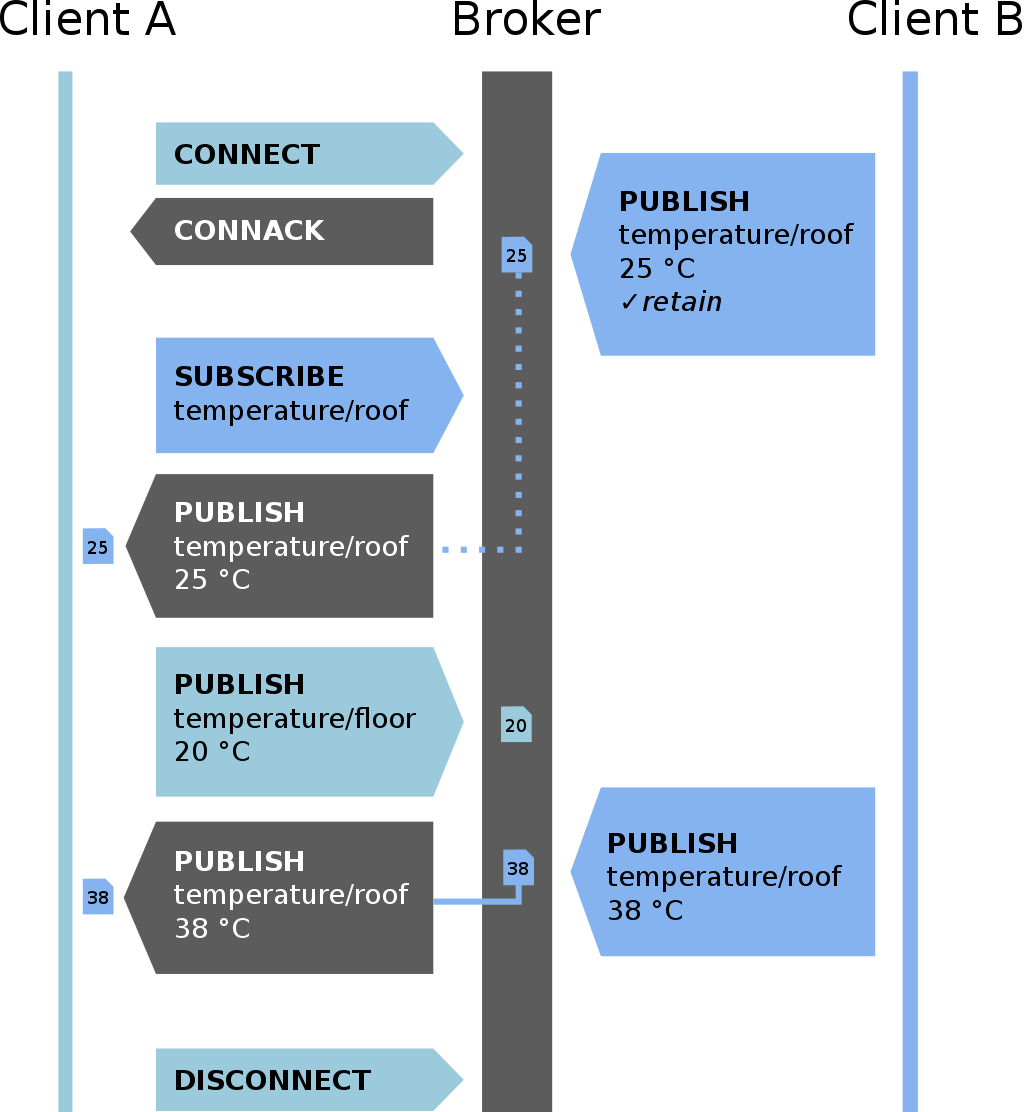
\includegraphics[width=0.9\textwidth]{img/mqtt_schematic.png}
            \caption{Schemat działania protokołu MQTT}
            \label{fig:mqtt_schematic}
        \end{figure}
         
        
    \section{Typy wiadomości}
        Istnieje obsługiwanych 14 typów wiadomości.
        
        \begin{itemize}
            \item CONNECT - Nawiązanie połączenia,
            \item CONNACK - Potwierdzenie nawiązania połączenia,
            \item PUBLISH - Publikacja wiadomości,
            \item PUBACK - Potwierdzenie publikacji wiadomości
            \item PUBREC - Potwierdzenie otrzymania wiadomości,
            \item PUBREL - Potwierdzenie wysłania wiadomości,
            \item PUBCOMP - Potwierdzenie końca publikowania wiadomości,
            \item SUBSCRIBE - Subskrypcja tematu,
            \item SUBACK - Potwierdzenie subskrypcji,
            \item UNSUBSCRIBE - Anulowanie subskrypcji,
            \item UNSUBACK - Potwierdzenie anulowania subskrypcji,
            \item PINGREQ - Żądanie PINGU,
            \item PINGRESP - Odpowiedź na żądanie PINGU,
            \item DISCONNECT - Zakończenie połączenia.
        \end{itemize}
        
        
    
    \section{Implementacja i konfiguracja}
      TODO docker, konfiguracja